\section{Linearisierung \formelbuch{76}}
	\begin{minipage}[c]{10cm}
		\subsection{LTI-Systeme \formelbuch{83}}
			\renewcommand{\arraystretch}{1.5}
			\begin{tabular}{|l|l|}
				\hline
				\textbf{Linearität} & \textbf{Zeitinvarianz}\\
				\hline
				$\Phi(x1+x2)=\Phi(x1)+\Phi(x2)$ & $\Phi(x(t-t_0)=\Phi(x)\cdot x(t-t_0)$ \\
				$\Phi(c\cdot x)=c\cdot \Phi(x)$ & \\
				\hline    
			\end{tabular}
			\renewcommand{\arraystretch}{1}
		\end{minipage}
		\begin{minipage}[c]{6cm}
			\subsection{Linearitätstest \formelbuch{80}}
			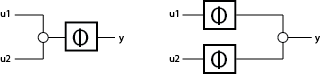
\includegraphics[width=6cm]{bilder/linearitaetstest}
		\end{minipage} \\
		
	Bei Gleichungen muss folgendes Unterschieden werden: \\
	\begin{multicols}{2}
	Linearität in den \textbf{Variablen} \\
	$y = \frac{a_0}{1-a_1} x_1 + a_0 x_2$ \\
	ist linear in den Variablen $x_i$, aber nicht in den Parametern $a_i$. \\
	
	Linearität in den \textbf{Parametern} \\
	$y = a_2 x^2 + a_1 \sin(2x) + 2.4 a_0$ \\
	ist linear in den Parametern $a_i$, aber nicht in der Variable $x$. \\
	\end{multicols}
	Die Gleichung $y=a_0 x_0+ a_1 x_1$ ist linear in Variablen und Parametern - 
	die Gleichung $y=x_0^{a_0}+x_1^{a_1}$ ist nicht linear.
	  	
	\subsection{Erwünschte Nichtlinearität \formelbuch{84}}
		In einem Prozess sind Linearitäten meist erwünscht, da sie meist mit
		Gleichungen zu lösen sind.
		Viele Efekte, wie zum Beispiel die Modulation oder so sind aber gerade erst
		durch Nichtlinearitäten möglich. Daher unterscheidet man:\\
	\begin{minipage}[c]{8cm}
		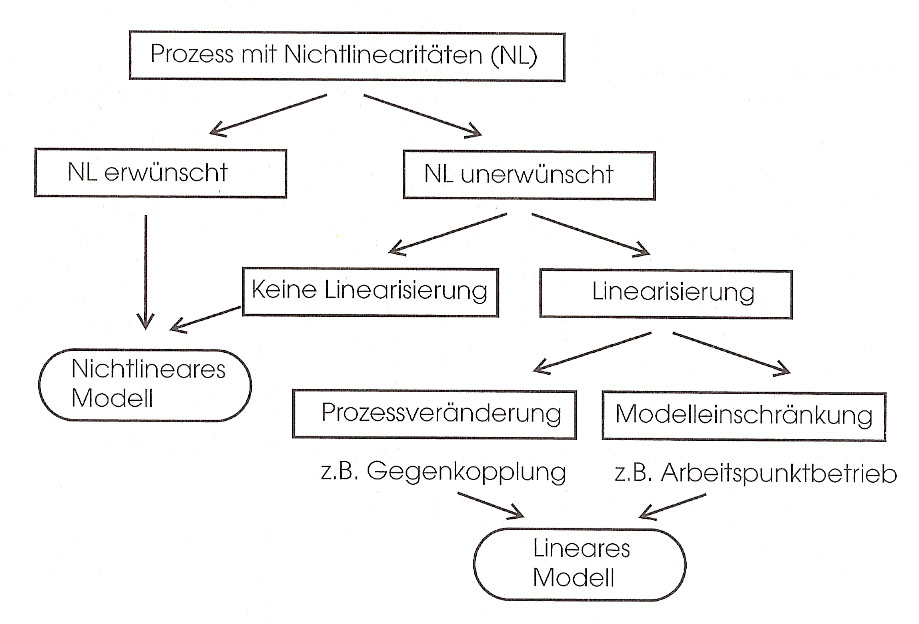
\includegraphics[width=8cm]{./bilder/Liste_Nichtlinearitaeten.jpg}
	\end{minipage}
	\begin{minipage}[c]{8cm}
		\textbf{Lineare Operationen} \\
		- Addition \\
		- Integration \\
		- Differentiation \\
		daraus folgt, dass folgende Glieder auch linear sind: \\
		- P-Glied \\
		- I-Glied \\
		- PT1-Glied
	\end{minipage}
	\subsection{Erfassen von nicht linearen Kurven}
	\subsubsection{Messung einer statischen Kennlinie \formelbuch{86}}
	\begin{minipage}{10cm}
		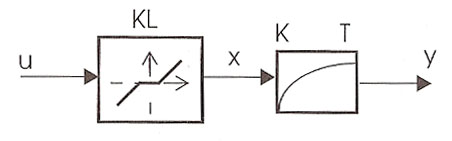
\includegraphics[width=7cm]{./bilder/NichtlinearMitPT1.jpg}   
    \end{minipage}
	\begin{minipage}{7cm}
    	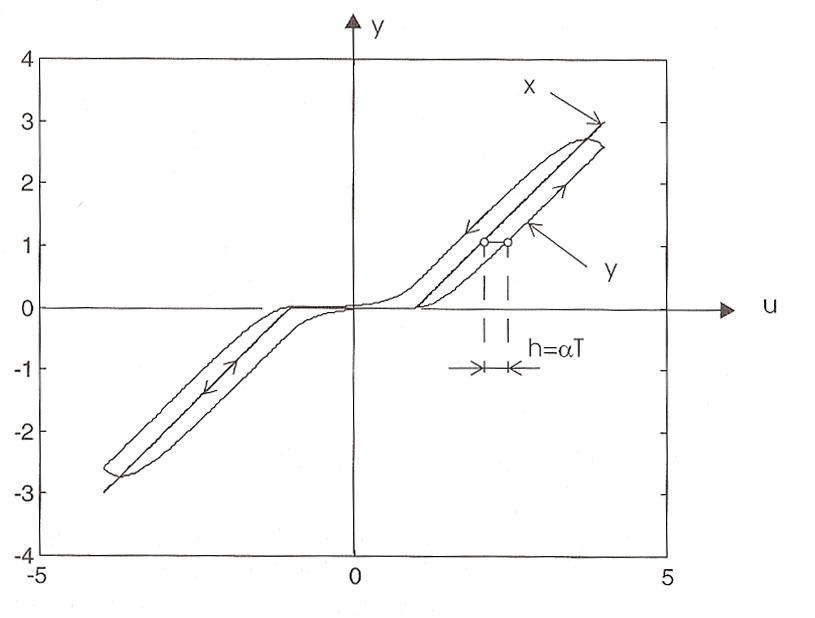
\includegraphics[width=5cm]{./bilder/NichtlinearMitPT1_dia.jpg}
    \end{minipage}\\
		Da das Signal x meist nicht zugänglich ist, muss man den ganzen Prozess
		ausmessen.\\
		Mit einem Dreieck kann man die Kennlinie auslesen. Sie wird jedoch von einer
		``unechten" Hysterese verzerrt, die eine Hysteresebreite von 2$\alpha$ T, wobei
		$\alpha$ die Rampensteilheit ist und T die Zeitkonstante des PT1-Gliedes.

	\subsubsection{Mathematische Erfassung einer Messkurve \formelbuch{89}}
	\begin{floatingfigure}[r]{12cm}
    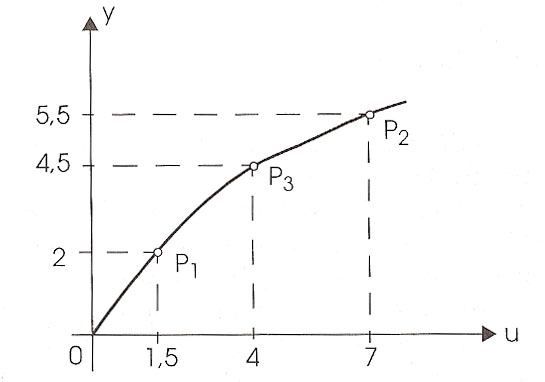
\includegraphics[width=10cm,height=3cm]{./bilder/KennlinieMitStuetzwerten.jpg}
	\end{floatingfigure}
   	
     	1. Wahl einer geeigneten Funktion:\\
     	Gesucht ist ein Graph, der eine ähnliche Form
		hat wie die Messkurve. Günstig sind Polynome, da sie mathematisch einfach zum
		beschreiben sind, aber auch Sinus- oder Arctan- Funktionen	\\ 
        \\
     	\begin{enumerate}[start=2]
        \item Bestimmung der Parameter:
          \begin{enumerate}
           \item Methode der ausgewählten Punkte:\\
          		\begin{enumerate}
                    \item Gleich viele Messpunkte wie frei zu wählende Parameter der
           			Approximationsfunktionen.
           			\item Einsetzen der Koordinaten der Messpunkte in die Gleichungen.
           		\end{enumerate}
           	\item Methode der kleinsten Fehlerquadrate:
           		\begin{enumerate}
                     \item Mindestens gleich viele Messpunkte wie Parameter der
           		Appxomationsfunktion, können jedoch mehr gewählt werden.
           		\item Fehler bilden zwischen Messpunkt und Funktionspunkt. zB.\\
           		P1:  $e_1=2-y=2-(a(1.5)+b(1.5)^2)$\\
           		P2:  $e_2=5.5-y=5.5-(a(7)+b(7)^2)$\\
           		P3:  $e_3=4.5-y=4.5-(a(4)+b(4)^2)$\\
           		\item Nach Gauss ist die beste Näherung, wenn die Summe der
           		Fehlerquadrate minimal wird. \\
           		$\Longrightarrow$ S =$ e_1^2+e_2^2+e_3^2=min$\\
           		$\frac{\delta S}{\delta a}=
           		2 e_1 \frac{\delta e_1}{\delta a}+
           		2 e_2 \frac{\delta e_2}{\delta a}+
           		2 e_3 \frac{\delta e_3}{\delta a}=0$\\
           		$\frac{\delta S}{\delta b}=
           		2 e_1 \frac{\delta e_1}{\delta b}+
           		2 e_2 \frac{\delta e_2}{\delta b}+
           		2 e_3 \frac{\delta e_3}{\delta b}=0$\\
           		\item Nachteil dieser Methode ist, dass es meist einen grossen
           		Rechenaufwand ergibt. Sie ist jedoch genauer als die erste Methode.
           		Ausserdem geht die Approixmationsfunktion nicht durch die Messwerte.
           		\end{enumerate}
		\end{enumerate}
	\end{enumerate}
	
\newpage

	\subsection{Linearisierung}
		\subsubsection{Modelleinschränkung \formelbuch{92}}
			Praktisch alle physikalische Systeme unterliegen gewissen Aussteuergrenzen.
			In diesen können sie linear sein. Es muss darauf achten, dass  das System
			diese nicht überschreitet. \\
			z.B. Festwert-Regelung: Die Kennlinie wird nur beim Einschalten durchlaufen.
			Ab dann bewegt sich die Regelung nur in einem sehr kleinen Bereich um den
			Arbeitspunkt, wo die Kennlinie linearisiert werden kann. \\
			
		\subsubsection{Arbeitspunkt \formelbuch{93}}
			Wenn eine Kennlinie für einen bestimmten Aussteuerung einen nicht zu grosse
			Krümmung hat, kann man in der Näherung diese durch die Tangente ersetzen, und
			somit wieder linear rechnen. \\
			Trigonometrische Funktionen bei Arbeitspunkt $\alpha = 0$: $\qquad \sin \alpha \approx
			\alpha \qquad \tan \alpha \approx \alpha \qquad \cos \alpha \approx 1$ \\
			\textbf{Vorgehen} \\
			\begin{minipage}[c]{6cm}
				\includegraphics[width=6cm]{bilder/LinArbeitspunkt}
			\end{minipage}
			\begin{minipage}[c]{12cm}
				\begin{enumerate}
					\item DGL des Systems bestimmen
					\item Alle Signale darstellen als $u(t)=u_0+\Delta u,\,v(t)=v_0+\Delta v,\dots$
					\item Arbeitspunkte $u_0,v_0,\dots$ = stationärer Zustand bestimmen
					\item Signaländerungen $\Delta u, \Delta v, \dots$ linearisieren
							(Tangente an Kennline)
					\item DGL durch Signaländerungen darstellen.
					\item Blockschaltbild mit Signaländerungen darstellen (siehe links)
				\end{enumerate}
			\end{minipage}
			
		\subsubsection{Durch inverse Kennlinie \formelbuch{94}}
		\begin{minipage}{11cm}
			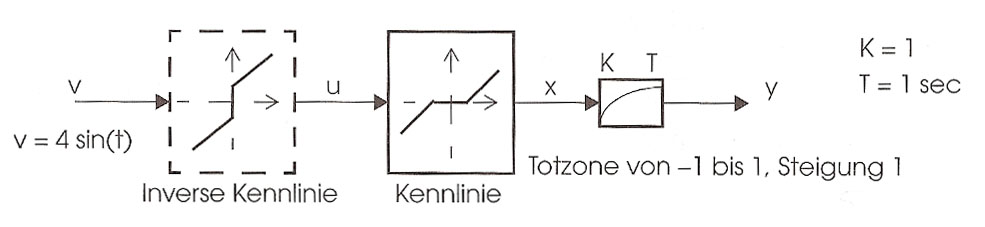
\includegraphics[width=10cm]{./bilder/Kennlinienkompensation.jpg}
        \end{minipage}
		\begin{minipage}{6cm}
        	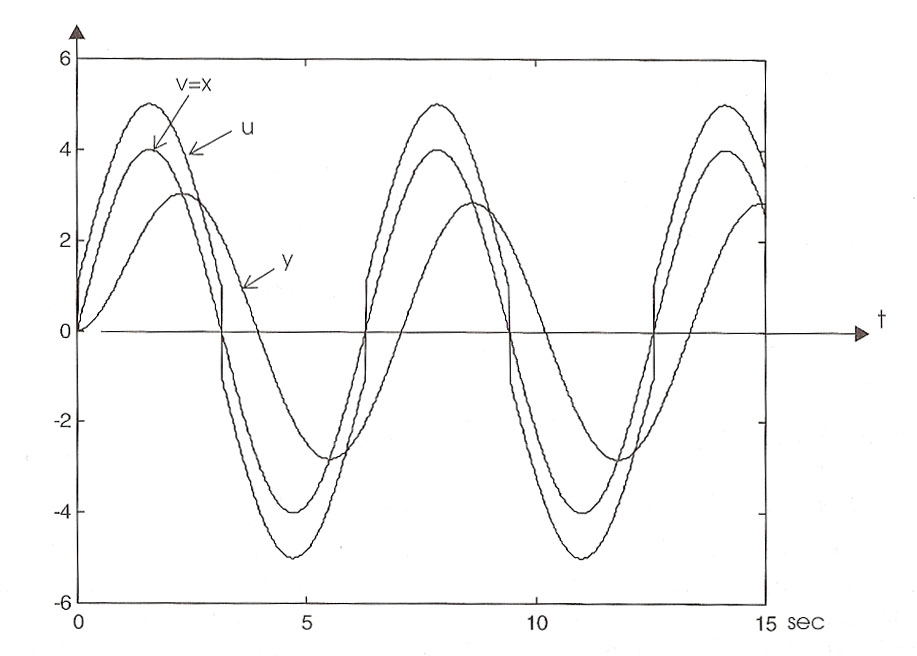
\includegraphics[width=6cm]{./bilder/Kennlinienkompensation_dia.jpg}
        \end{minipage}\\
			Durch das Vorschalten der Inversen Kennlinie kann man die Nichtlinearitäten
			beheben. Das System als ganzes reagiert nun linear, das Innere des System
			jedoch immer noch nicht, wie man an den Kennlinien gut erkennen kann.
			
		\subsubsection{Durch Gegenkopplung \formelbuch{96}}
				\begin{minipage}{11cm}
			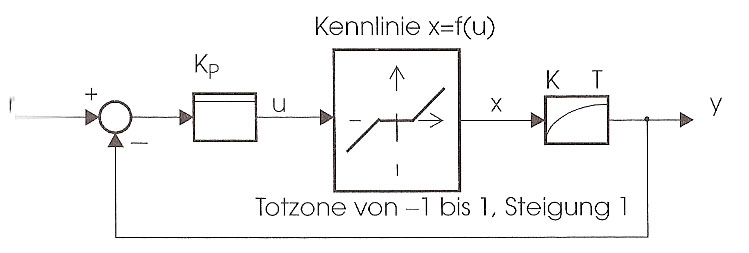
\includegraphics[width=10cm]{./bilder/Gegenkopplung.jpg}
        \end{minipage}
		\begin{minipage}{9cm}
        	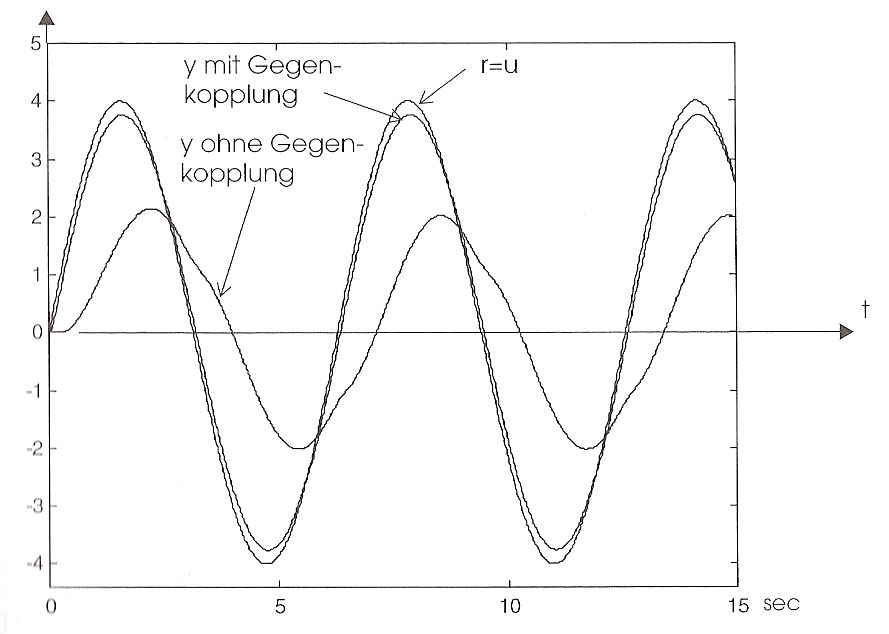
\includegraphics[width=6cm]{./bilder/Gegenkopplung_dia.jpg}
        \end{minipage}\\
			Da ein Prozess variierende Koefizienten besizten kann, kann die Kompensation
			nicht immer mit der inversen Kennlinie geschehen. Deshalb ist es oft
			günstiger die Nichtliniearitäten mit einer Gegenkopplung zu kompensieren.
			Diese ist umso wirksamer je grösser die Verstärkung $K_p$ ist.
			Es können jedoch Stabilitätsprobleme auftreten.
